\documentclass{article}
\usepackage[utf8]{inputenc}
\usepackage{graphicx}
\usepackage{hyperref}
\usepackage{amsmath,amssymb}
\usepackage{amsthm}
\usepackage[
backend=biber,
style=alphabetic,
sorting=ynt
]{biblatex}
\nocite{*} 
\addbibresource{bibliography.bib}
\hypersetup{
    colorlinks=true,
    linkcolor=blue,
    filecolor=magenta,      
    urlcolor=blue,
    citecolor={blue},
}
\graphicspath{ {images/} }
\addtolength{\oddsidemargin}{-.475in}
\addtolength{\evensidemargin}{-.475in}
\addtolength{\textwidth}{.95in}
\addtolength{\topmargin}{-.475in}
\addtolength{\textheight}{.95in}

\newtheorem{theorem}{Theorem}[subsection]
\newtheorem{corollary}{Corollary}[theorem]

\newtheorem{definition}[theorem]{Definition}
\newtheorem{remark}[theorem]{Remark}
\newtheorem{lemma}[theorem]{Lemma}

\newtheorem{proposition}[theorem]{Proposition}
\newtheorem{claim}[theorem]{Claim}
\newtheorem{observation}[theorem]{Observation}
\newtheorem{fact}[theorem]{Fact}
\newtheorem{assumption}[theorem]{Assumption}



\def\R{\mathbb{R}}
\def\E{\mathbb{E}}
\def\N{\mathbb{N}}
\def\set#1{\left\{ #1 \right\}}
\renewcommand{\|}{\;|\;}

\title{An Exploration of 33.$\bar{3}$\% Attack Vectors in Pure Proof of Stake}
\author{Aparna Krishnan, Zubin Koticha, Alexis Gauba, \and Maaz Uddin, Dev Ojha, Philip Hayes \\ \small{University of California, Berkeley} \\
\small{Blockchain Lab, Sutardja Center for Engineering and Technology} \\\small{Blockchain at Berkeley, Research and Development - Cryptoeconomics Research} \and \small{Special Thanks to Karl Floersch from the Ethereum Foundation, \and \small{\and \small Profs. Dawn Song, Gireeja Ranade, Satish Rao Department of EECS, UC Berkeley,
\and \small {Sankalp Aggarwal from Tendermint}}}}

\date{January 2018}

\begin{document}
\maketitle
\begin{abstract}
Proof of Stake (PoS) is a blockchain consensus protocol in which validators staking some amount of funds can both propose and vote on new blocks in the network. These validators command voting power proportional to the percentage of funds they have bonded. A key vulnerability of the PoS systems that we model is that, if a single validator reaches $\frac{1}{3}$ stake, the attack threshold, because someone with $\frac{1}{3}$ stake has the ability to prevent network consensus. In this paper, we conduct an examination of the possibility of a validator reaching the attack threshold in the network via two methods.  

We first examine the Superior Returns Attack Threshold (SRAT) method, in which a member of the network increases her ownership of tokens through investing in high-risk, high-return securities until she has sufficient wealth that when she stakes her wealth, she will command an attack stake. We next inspect the Random Attack Threshold (RAT) method, whereby a validator unintentionally accumulates an attack stake through stochastic randomness. 

In the first case, we show that there is a non-zero probability of a validator obtaining $\frac{1}{3}$ stake when intentionally trying to do so, which may pose potential challenges to the security of pure PoS, but in the second case, we show that there is a near zero probability of a validator obtaining $\frac{1}{3}$ stake through stochastic randomness with constant rewards. 

\end{abstract}

\section{Introduction}

\subsection*{Proof of Work and Proof of Stake:}

Cryptocurrencies like Bitcoin have been gaining note recently for distinct benefits they offer over fiat currency including increased transparency among other parameters \cite{BitcoinFAQ}. These currencies are backed by distributed ledgers known as blockchains. The computers that secure these blockchains are known as miners. These miners have a monetary incentive to come to  consensus with other miners regarding the ledger's history. This process referenced as Nakamoto Consensus in the space, which is backed by a process known as Proof of Work (PoW) \cite{Bitcoin.org}.\\ \\ Proof of Work is wasteful of energy and computational power, slowing down the network considerably. Proof of Stake (PoS) has been proposed as an alternative blockchain consensus protocol. Proponents argue that PoS resolves challenges with Proof of Work such as energy inefficiency, high latency, and centralization risk, to name a few \cite{EthPoSFAQ}. PoS has been in development for major networks such as Ethereum, NEO, and Tendermint among others due to the strong arguments in its favor,  \cite{EthPoSFAQ}. \\ \\ In a PoS system, consensus is reached through the agreement of validators who have bonded their coins to the network. These validators are akin to miners in PoW. However, in PoS, validators create a deposit (a bond) of coins which allows them to propose and vote on new blocks. In some iterations of PoS (BFT-style), one of these validators is randomly chosen as a proposer to propose a new block to add to the blockchain in every round\cite{EthPoSFAQ}. The rest of the validators vote on the inclusion of this new block, with voting power in proportion to the bonds they have staked. Consensus is achieved when the 66\% of validators agree on accepting the new block . \newline \newline The PoS system we examine is one in which a proposer is chosen from among the validators with a likelihood proportional to the funds they have bonded in the network \cite{EthPoSFAQ}. PoS depends on both rewards and penalties to incentivize agents in the system to act honestly. The analyses in this paper are inspired by BFT-style PoS.

\subsection*{Motivation (the Problem of $\frac{1}{3}$):}

In traditional PoW blockchains, a malicious actor with 51\% of mining power can rewrite the history of the blockchain, and thus 51\% is considered the security threshold of a PoW blockchain \cite{nakamoto2008}. \\ 

\noindent Brewer's CAP Theorem posits the trade-offs between consistency and availability in a distributed system \cite{Brewer}. To find a balance between consistency and availability, the PoS system we model can tolerate up to $\frac{1}{3}$ byzantine faults \cite{Brewer}. Given that voting power in PoS is proportional to the number of staked tokens one has bonded, at $\frac{1}{3}$ stake an attacker can refuse to finalize any further blocks, or censor the network to their specific views by refusing to finalize specific blocks of their choosing \cite{EthPoSFAQ}.  Malicious validators can also indefinitely stall consensus, by not approving any new blocks at all. As such, it's important to decrease the likelihood of any validator commanding $\frac{1}{3}$ of the total staked tokens. While an attack can be mitigated by a hard fork, in which the network split can undo malicious behavior, such a solution is economically and socially costly, and undermines trust in the blockchain \cite{Buterin2016}. Therefore, in PoS, preventing any single validator gaining enough stake to undermine consensus is a paramount issue for the network. As such, it's important to decrease the likelihood of any staker to commanding $\frac{1}{3}$ of the total staked tokens. \newline 
 
\noindent In this paper, we analyze the difficulty of a validator obtaining $\frac{1}{3}$ stake. We look at two possibilities of reaching $\frac{1}{3}$ stake. The first case is the Superior Returns Attack Threshold, in which a member of the network becomes sufficiently wealthy through high returns that when she decides to stake her wealth, she has enough for an attack stake. The second is the Random Attack Threshold; a case wherein a validator gets to $\frac{1}{3}$ through stochastic randomness. 

\subsection*{Reward Scheme for our PoS:}
We model a PoS system in which a proposer is chosen from the set of validators to compose a block upon which other validators vote. If a validator has bonded $X$\% of all staked tokens, then that validator will be chosen as the next block proposer with $X$\% likelihood. When a user of the blockchain proposes a transaction, the user includes a transaction fee, all of which is credited to the block proposer. Then validators vote on each proposed block. Each validator, including the proposer, receives a small validation reward for voting on each block, and the validation reward is proportional to the validator's stake. \\

There are three mechanisms by which the protocol can incentivize honest behavior in PoS:
\begin{itemize}
    \item Transaction Fees: These transaction fees disincentivize block proposers from including empty blocks, prevent users from spamming the network with trivial transactions, and provide a mechanism for block proposers to order transactions.
    \item Validation Rewards: Validation rewards are given to all validators who sign off on a block. This both incentivizes ETH holders to become validators, and incentivizes existing validators to be available to sign each block. Note that these validation rewards must be paid proportional to validators' stake.
    \item Punishments: There are a subset of punishments, some of which (e.g. slashing) are only levied on actors that are acting in a demonstrably malicious manner, and others which may be levied on honest actors when the source of malice is uncertain (e.g. data unavailability punishments).
\end{itemize}

\subsection*{Superior Returns Attack Threshold (SRAT):}
Validators expect to get some return for their validation, $r_{v}$, from staking their tokens on the network via their share of validation rewards and transaction fees. If some ETH holder ${A}$ decides to not to stake her tokens, and instead invests these in another asset $hr$ which has higher risk than validation, but also has a higher expected rate of return $r_{hr} > r_{v}$, she can expect on average to grow her wealth at a faster rate than bonded validators. If she, in fact, does receive a higher return, she can potentially accumulate sufficient ETH that when she decides to stake her tokens, she has a stake over $\frac{1}{3}$.

\subsection*{Random Attack Threshold (RAT):}
In this system, the stake of any validator with $x\%$ of bonded funds $< 33\%$, will be expected to remain at $x\%$ staked at any later time ${t}$ given the following: 
\begin{itemize}
  \item All validators restake all their rewards
  \item No validators unbond their stake
  \item No other users stake, so no one is added to validator set
\end{itemize}

Note that proposers collect both transaction fees and validation rewards, while other validators collect only validation rewards. Since a proposer is selected at random from the group of validators, it is possible that one validator $B$ is selected as the proposer much more often than others. Assuming $B$ immediately restakes her income, her wealth will grow with a higher rate of return than other validators, and it is possible over time that this increases her stake to $\frac{1}{3}$. \\

We model the case of a validator probabilistically obtaining an attack stake using a P\'olya's Urn model. \\

Before we analyze the SRAT and RAT methods, let us examine the rewards scheme in more depth, specifically the awards for proposers and other validators in this scheme. 


\subsection{Rewards Scheme - Awards for Proposers vs. other Validators:}

We argue that block proposers must get rewards for each block at least as large as those of a validator possessing the same stake. This helps to prevent large stakers from forming multiple bonded Sybil identities.\\ \\
We demonstrate that stakers have a strong incentive to break their stake into Sybil identities in the case that validation rewards are not paid to block proposers through the following example:\newline \newline
Consider a user who bonds her tokens, which amount to x\% of all staked tokens, through one single account, she then has an x\% likelihood of being chosen as block proposer.
\begin{enumerate}
  \item In Case 1, if she is not chosen as a  proposer, she receives x\% of the validation rewards. If she is chosen to be a proposer, she receives transaction fees from that block but misses out on validation rewards.
  \item In Case 2, if she is not chosen to be the block proposer, she receives x\% of validation rewards, similar to Case 1. However, unlike in Case 1, if she is chosen to be a proposer, she receives transaction fees from that block \textit{as well as} x\% of the validation rewards
\end{enumerate}\newline \newline

She would respond to Case 1, a design lacking validation rewards to block proposers, by forming Sybil identities: since she would not be getting x\% of validation rewards when chosen as a block proposer, she would have been better off splitting her x\% into ${k}$ accounts each with $\frac{x}{k}\%$ of total staked tokens. This maintains her likelihood of being chosen as block proposer at  x\%. However, when she is chosen as a proposer, her other accounts will still deliver $x-\frac{x}{k}\%$ of validations rewards to her for that block. As ${k}$ becomes larger, in the case the probability of her being chosen as block proposer remains constant while she increases her share of validation rewards.\newline \newline
We want to prevent Sybil identities because increasing the number of distinct accounts staked will increase network latency \cite{buterin17}. An increase in network latency would result in discrepancies in information disseminated to the validator pool, in that not all validators would hear about a specific block, leading to both inefficiency and inconsistency within the network \cite{Kwon2016}.

\section{Superior Returns Attack Threshold (SRAT)}

\subsection{Sketch of a SRAT:}
A risk-tolerant attacker with some wealth of Ether $w < 33$\% of all staked tokens invests in some Ethereum-based financial asset that offers a greater return than staking, until the attacker exceeds $\frac{1}{3}$ of staked tokens and can effectively control consensus.\newline
\subsection{How to obtain SRAT:}
A user can increase her wealth by investing and obtaining superior returns; these  returns may be  accumulated either off-chain or on-chain. As of now, superior returns are commonly earned off-chain (in fiat currency). There are two ways in which the network can stay protected from off-chain wealth. The first situation is if the staking currency becomes increasingly expensive in terms of fiat currency. A second method we propose is to make the supply of tokens inelastic by making sure that a minimum percentage of staked tokens remains locked at any given time, with a penalty fee being charged for unbonding before the end of the staking period.\newline \newline
While currently superior returns are usually available only off-chain, this is likely to change. Blockchain platforms designed for smart-contracting, such as Ethereum, will eventually allow for a wide variety of securities to be trustlessly traded on-chain. Some of these investment classes will provide higher expected returns (and higher risk) than the low-risk validation rewards and transaction fees provided by staking. Thus, if an investor is able to purchase assets with expected returns (and risk) greater than those of being a staker, then the investor may be able to grow her money faster than bonded stakers, if her realized returns are indeed higher than those for stakers. If so, eventually she can obtain sufficient wealth to be able to stake it and get control over $\frac{1}{3}$ of the network's total stake. (As the security is denominated in Ether, it can readily be sold and the Ether can be restaked, as opposed to a dollar-denominated security that would have to be exchanged for dollars and then for Ether.) \newline \newline
According to the Capital Asset Pricing Model, in an efficient market, assets with greater risk associated with them must provide a higher rate of expected rewards \cite{sharpe1964}. Since many new blockchains, such as Ethereum, provide the flexibility to allow for a wide variety of different investment types on chain, in the long run, there should exist some security in the Ethereum ecosystem which provides an expected return greater than rewards gained by validation, at a greater level of risk. That is, if bonding as an honest validator provides expected reward $r_{v}$ and expected punishment $p_{v}$ (a function of unavailability punishments) over some distinct time period, there exists some high-risk security which provides some superior expected return $r_{hr} = r_{v} - p_{v} + \varepsilon$ (where $\varepsilon > 0$) over the same time period.\newline \newline
Let's say an investor begins with a certain amount of wealth that, were she to stake at the beginning, would give her a stake of $x_{0}$ (as a percentage of the total bonded stake). Let's say that, instead of staking this initial wealth, she invests in the high-risk asset. Then $x_{N}$, the percentage amount of stake she could possess after $N$ time periods is given by:
\begin{equation}
x_{N} = x_{0} * (1 + r_{hr})^N 
\end{equation}
or
\eq\begin{equation} 
x_{N} = x_{0} * (1 + r_{v} - p_{v} + \varepsilon)^N
\end{equation}\newline 
This is assuming that all stakers rebond their validation earnings and that no other Ether gets bonded or unbonded. The expected amount of time it would take an attacker with x\% of stake to obtain 1/3 stake is therefore N periods as demonstrated by the following equation:
\begin{equation}
\frac{1}{3} *  100 * (1 + r - p)^N  = x * (1 + r - p + \varepsilon)^N   
\end{equation}
Solving for N, the expected amount of time it would take a user to get to $\frac{1}{3}$ stake:
\begin{equation}
N = \frac{\ln{(100)}- \ln{3x}}{ \ln{(1 + r -p + \varepsilon)} - \ln{(1 + r - p)}}
\end{equation} \newline 

In this case, as long as the return on these high risk investments is less than or equal to the return provided by staking, being a staker is preferable since it provides an equivalent or greater risk-free rate of return. However, if the return from the risky asset is greater, a risk-tolerant attacker would potentially be incentivized to purchase that asset and thus accumulate tokens, which they could then stake. \newline


\subsection{Difficulty of such a SRAT:}

It is unclear that such returns as below are reasonable on Ethereum, but are provided as a rough exercise to see what would happen if Ethereum rewards matched those that are expected for USD assets. \newline\newline Since the annualized return of the S&P500 has averaged around 10\% for the last 90 years \cite{Snider}, the future amount of Ether invested at a comparable rate for N years is:
\begin{equation}
FV_{ETH} = PV_{ETH} * (1.1)^N
\end{equation}
(Again, it is not clear that you'd be able to attain a 10\% annualized Ether return, even if you would be able to get a 10\% annualized dollar return.)\newline

Assuming the following: 
\begin{itemize}
\item Staked Ether grows at a rate $r_{v} < 10\%$ due to validation rewards and transaction fees
\item A party commands $x\%$ of the initial Ether
\item No new individuals enter or exit the validator set
\item All validators restake their new earnings
\end{itemize}
Then we see that the time until that party commands $\frac{1}{3}$ of the total staked amount is:

\begin{equation}
\frac{1}{3} * 100 * (1 + r)^N  = x(1.1)^N
\end{equation}

Solving for $N$,  we see:
\begin{equation}
N = \frac{\ln{(100)}- \ln{(3x)}}{ \ln{1.1} - \ln{(1+r)}}
\end{equation} \newline The risk-free rate (1-yr treasury note) is 1.4\% currently. Assume that validation rewards are exactly 1.4\%. An attacker starting with 10\% of the total staked tokens will thus command $\frac{1}{3}$ of the network in 6.27 years.

\begin{equation}
    N =  \frac{\ln{(100)} - \ln{(60)}}{\ln{1.1}- \ln{1.014}}
\end{equation} \newline Assuming she invests in leveraged assets, such as 2x leveraged S&P500 (by margin trading), she can approach 20\% returns. An attacker would own $\frac{1}{3}$ of staked tokens in 3.03 years in this case.

\begin{equation}
    N =  \frac{\ln{(100)} - \ln{(60)}}{\ln{1.2}- \ln{1.014}}
\end{equation} \newline From the above we can deduce the following:
\begin{itemize}
  \item To protect the network, we need to Maximize N:
    \begin{equation}
    \frac{1}{3} * (100 - x)(1 + r - p)^N  = x * (1 + r - p + \varepsilon)^N
    \end{equation}
  \item Accordingly, the following must hold true: 
        $r - p > 0$
\end{itemize}

\subsubsection*{Takeaway:}

Two arguments often used in favor of PoS are:
\begin{itemize}
    \item As a wealthy actor tries to “corner the market” on ETH  through purchasing more, she will find herself paying more for each additional ETH she buys. 
    \item As any malicious validator approaches $\frac{1}{3}$ of the total share of staked tokens, the members of the network will respond by bonding their ETH and joining the validator set, so that they can dilute the attacker’s share and prevent a $\frac{1}{3}$ attack.
\end{itemize}
However, this type of attack may call into question the validity of those two arguments. As the Ethereum ecosystem develops, eventually individuals will be able to invest in on-chain assets and earn ETH-denominated returns to their existing ETH. Therefore, a wealthy actor never needs to ‘buy’ her way into the network; she simply needs to invest at some high-reward ETH-denominated interest-rate. While is it not guaranteed that she will, indeed, recieve the high returns needed to obtain the wealth required for an attack stake (given the higher risk of her assets), it is quite likely that she, or some other attacker, will be ultimately able to achieve such wealth. \\ 

Further, a big problem with this kind of attack is that as any actor accumulates additional ETH, she is reducing the rest of the network’s ability to bond more tokens in order to dilute their stake. That is, since there is a fixed supply of tokens which can be earned from external non-validation activities, as an actor gains their 20\% returns, that actor is simultaneously reducing the token share of others. Therefore, the rest of the network has less ETH to add to the validator set in order to prevent a $\frac{1}{3}$ attack.

\section{Random Attack Threshold (RAT) \\ Probability of Reaching $\frac{1}{3}$ through Randomness:}
One way to reach $\frac{1}{3}$ stake is through stochastic randomness in that there is a small likelihood that validators could be repeatedly chosen to select a block, collect transaction fees, immediately restake rewards, and continually increase their fractions of the network's total deposit until they reach $\frac{1}{3}$. Thus we analyze the probability of any validator reaching this $\frac{1}{3}$ threshold. \\ \\ Here, we consider a simplified version of a typical Proof-of-Stake protocol in which we have $m$ validators. Since we are mostly concerned with local dynamics in this particular discussion, we will assume that the number of validators remains fixed over time and there is no external capital in or out flow, i.e., no validators bond additional stake or cash out their stake. Our abstract process proceeds as follows: at every round, a single validator is chosen with probability equal to their proportion of staked tokens. If a validator is chosen, then they receive a reward of some constant number of staking tokens. For the purposes of simplification we consider the reward to be $1$ token. The general case for a reward of $r$ tokens can easily be derived from this simplification. We examine how long it takes until any validator’s proportion of the tokens passes the byzantine threshold.


\subsection{Constant Reward Polya Urn}
The Proof-of-Stake process lends itself quite naturally to an urn model in which we view the validators as different-colored balls in an urn. The number of $i^{th}$ colored balls in the urn is then equal to the number of staking tokens owned by the $i^{th}$ validator.
\begin{center}
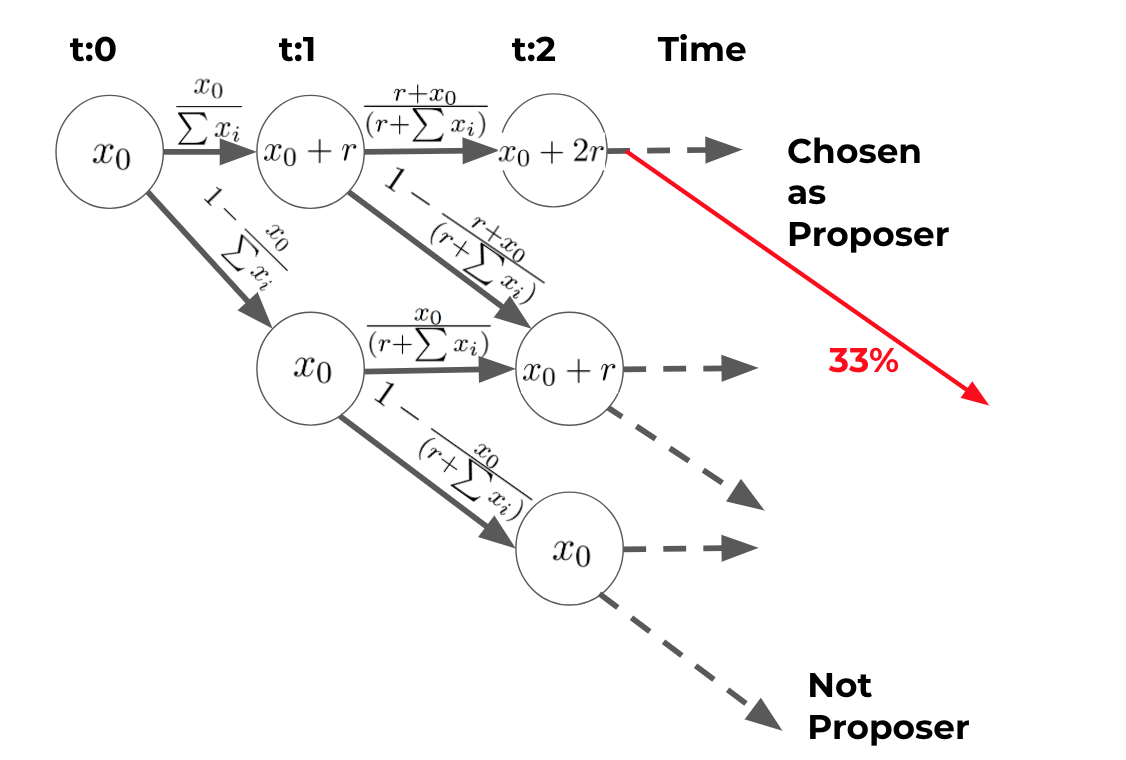
\includegraphics[scale=0.4]{Markov.png}
\newline State Transition Diagram
\end{center}
The above state transition diagram is a visualization of the different stakes of the $0^{th}$ validator which we simulate with a P\'olya Urn Model. We model a state transition diagram where each state represents the number of tokens staked. At time $t = 0$ the validator has $x_0$ number of tokens staked. The probability the $0^{th}$ validator gets chosen to be a proposer is $\frac{x_0}{\sum x_i}$ at $t = 0$ where $x_i$ is the number of tokens the $i^{th}$ validator has deposited. The probability that the $0^{th}$ validator is not chosen to be a proposer is $1 - \frac{x_0}{\sum x_i}$ at $t = 0$. 

\subsection*{Definitions}
A P\'olya urn is an urn containing balls of up to $K$ different colors, where $K>=2$. The urn evolves in discrete time steps - at each step, one ball is sampled uniformly at random; The color of the withdrawn ball is observed, and the ball is returned to the urn. In addition, a ball of the same color as the ball that was drawn is added to the urn. 
\newline \newline
In section 4.1, we consider a P\'olya urn with $m$ validators. Let the composition of the validator set at time $t$ be represented by the vector $X_t = (x_t^{(1)},..., , x_t^{(m)})$ where  $x_t^{(i)}$ is the stake (number of tokens) of the $i^{th}$ validator at time $t$. We consider a distribution after we simulate the process for $n$ rounds. $y_j$ is the number of times the $j^{th}$ validator wins in the $n$ rounds. Let $\Gamma_0$ be the total stake at the start in the urn.
\begin{equation*}
        \Gamma_0 = \sum_{i = 1}^{m}{x_0^{(i)}}
\end{equation*}

Notations:
\begin{itemize}
    \item $\langle x \rangle_n = x(x + 1)..(x + (n - 1)) $
    \item $Y[j]$ is the $j^{th}$ element of the $Y$ vector.
    \item ${n \choose y_1,.., y_m} = \frac{n!}{y_1!*..*y_m!}$
\end{itemize}

\subsection{Convergence of the Distribution}
\begin{theorem}
Let $p_n^{(i)} = \frac{x_n^{(i)}}{\sum_{j = 1}^{m'}x_n^{(j)}}$, be the proportion of stake of the $i^{th}$ validator after $n$ rounds. Let $\mathcal{F}_n =  \sigma{(v_i)}$, where $v_i$ is the $i^{th}$ validator. Then $p_n^{(i)}$ is a Martingale w.r.t $\mathcal{F}_{n-1}$
\end{theorem}
\begin{proof}
\begin{equation*}
    E[p_n^{(i)}|\mathcal{F}_{n-1}] = E[\frac{x_n^{(i)}}{\sum_{j = 1}^{m'}x_n^{(j)}}|\mathcal{F}_{n-1}] = E[\frac{x_n^{(i)}}{\sum_{j = 1}^{m'}x_0^{(j)} + n}|\mathcal{F}_{n-1}] 
\end{equation*}
\begin{equation*}
    = \frac{1}{\sum_{j = 1}^{m'}x_0^{(j)} + n} E[x_n^{(i)}|\mathcal{F}_{n-1}] =  \frac{1}{\sum_{j = 1}^{m'}x_0^{(j)} + n}(x_{n-1}^{(i)} + \frac{x_{n-1}^{(i)}}{\sum_{j = 1}^{m'}x_{0}^{(j)} + n - 1}) = p_{n-1}^{(i)}
\end{equation*}
\end{proof}

The takeaway from the above theorem is that since $p_n^{(i)}$ is a martingale and is bounded by 1 on the upper end, it must surely converge to some value.
\subsection{Distribution and Expected Value for a Constant Reward}

\begin{theorem}
Suppose a P\'olya urn starts with an initial composition of $X_0$ and initial total stake $\Gamma_0$. Let $X_n$ be the composition of the P\'olya urn after $n$ draws, then
\begin{equation}
    P(x_n^{(j)} = x_0^{(j)} + y_j, j = 1,..,m) = \frac{\prod_{j=1}^m{\langle x_0^{(j)}\rangle_{y_j}}}{\langle \Gamma_0 \rangle_n} {n \choose y_1,..,y_m}
\end{equation}
\end{theorem}
\begin{proof}
If the $i^{th}$ colored ball is drawn $y_i$ times, then $x_0^{(i)}(x_0^{(i)} + 1) .. (x_0^{(i)} + y_i - 1)$ is in the numerator in some ordering. Thus independent of ordering the numerator will remain $\prod_{j=1}^m{\langle x_0^{(j)}\rangle_{y_j}}$ and $\langle \Gamma_0 \rangle_n$ will be in the denominator. There are ${n \choose y_1,..,y_m}$ ways of ordering the distribution in the numerator.
\end{proof}
\noindent Using Theorem 4.3.1, we can calculate results like the expected value vector and the probability of any validator reaching a certain threshold after $t$ steps.

\subsubsection{Calculating the probability that someone in the network reaches the threshold}
Let $v_i$ be the $i^{th}$ validator and $V$ be the set of all validators. $S(v_i)$ be the set of events such that the $i^{th}$ validator crosses the threshold. Let $P(v_i)$ be the probability that the $i^{th}$ validator crosses the threshold. Let $z_i$ be the minimum number of times the $i^{th}$ validator would have to be chosen to reach the threshold $p$ ($p$ is a proportion like $\frac{1}{3}$) in $n$ rounds. 
$$\frac{x_0^{(i)} + z_i}{\Gamma_0 + n} \geq p$$
\begin{equation}
z_i = \lceil p*(\Gamma_0 + n) - x_0^{(i)}\rceil
\end{equation}
We can model the probability of each validator $v_i$ reaching a certain threshold by considering a 2 validator system - the first being validator $v_i$ and the second being all the other validators. 
\begin{corollary}
    The probability of a single validator $v_k$ crossing the given threshold after $n$ rounds is:
\begin{equation}
    \frac{\sum_{i = z_k}^{n} \binom{n}{i} \langle x_0^{(k)} \rangle_i \langle \Gamma_0 - x_0^{(k)} \rangle_{n-i}}{\langle \Gamma_0 \rangle_n}
\end{equation}
\end{corollary}

\begin{corollary}
The probability of an index set $S$ of the $m'$ validators such that $m'<= m$, all reaching the threshold $p$ after $n$ rounds is represented by $ P(\frac{x_n^{(S_k)}}{\Gamma_n} >= p, k = 1..m')$
\begin{equation}
  = \frac{
    \sum_{i_1=z_{S_1}}^{n - \sum_{k=1}^{m'} z_{s_k}} \sum_{i_2=z_{S_2}}^{n-i_1} \ldots \binom{n}{i_1,i_2,.., i_{m'}} \langle x_0^{(S_1)} \rangle_{i_1} \langle x_0^{(S_2)} \rangle_{i_2} ..\langle x_0^{(S_{m'})} \rangle_{i_{m'}}}{\langle \Gamma_0 \rangle_n}
\end{equation}
\end{corollary}

\begin{corollary}
The probability that any validator crosses the given threshold $p$ is represented by $    \frac{\left\|\bigcup\limits_{i=1}^{m} S(v_i)\right\|}{\left|S(U)\right|} $
\begin{equation}
 = \sum_{i=1}^{m} P(\frac{x_n^{(i)}}{\Gamma_n} >= p) - \sum_{i=1}^{m} \sum_{j=1}^{m-i} P(\frac{x_n^{(i)}}{\Gamma_n} >= p \And \frac{x_n^{(j)}}{\Gamma_n} >= p)  + \sum_{i=1}^{m} \sum_{j=1}^{m-i} \sum_{k=1}^{m-i-j} P(\ldots)
\end{equation}
\end{corollary}
\noindent Each successive term should be significantly smaller than the previous term. For $Threshold = \frac{1}{2}$, there is only one term, since when there are more than two validators, it is impossible for two validators to each have $\frac{1}{2}$ of the total stake. Similarly, for $Threshold = \frac{1}{3}$ you only need the second order approximation. 

\begin{center}
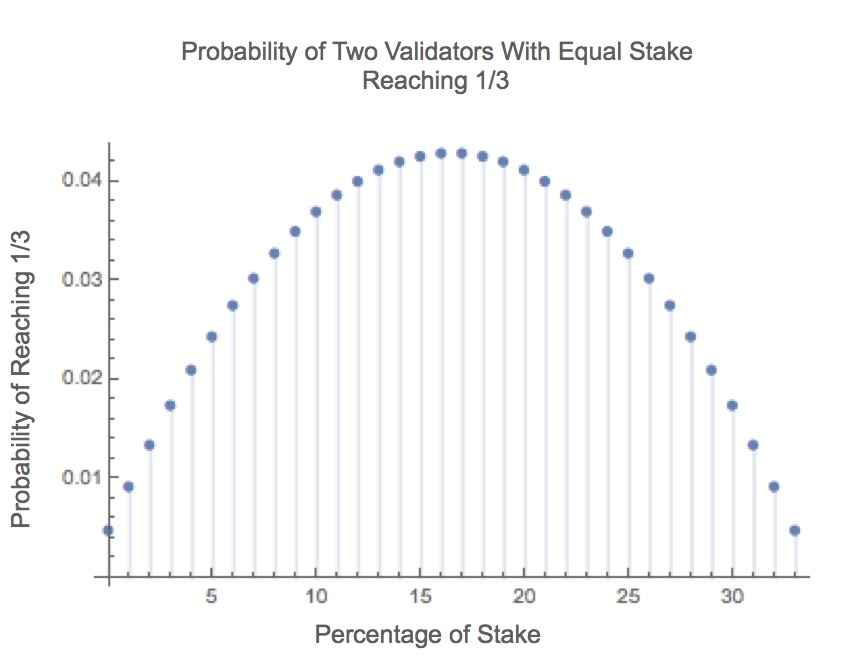
\includegraphics[scale=0.3]{images/2EqVal.jpg}\newline\caption{Beta Binomial Distribution (probability density graph) conveying the probability of validator one reaching $\frac{1}{3}$ stake, when the two validators begin with equal stake.}
\end{center}

\begin{center}
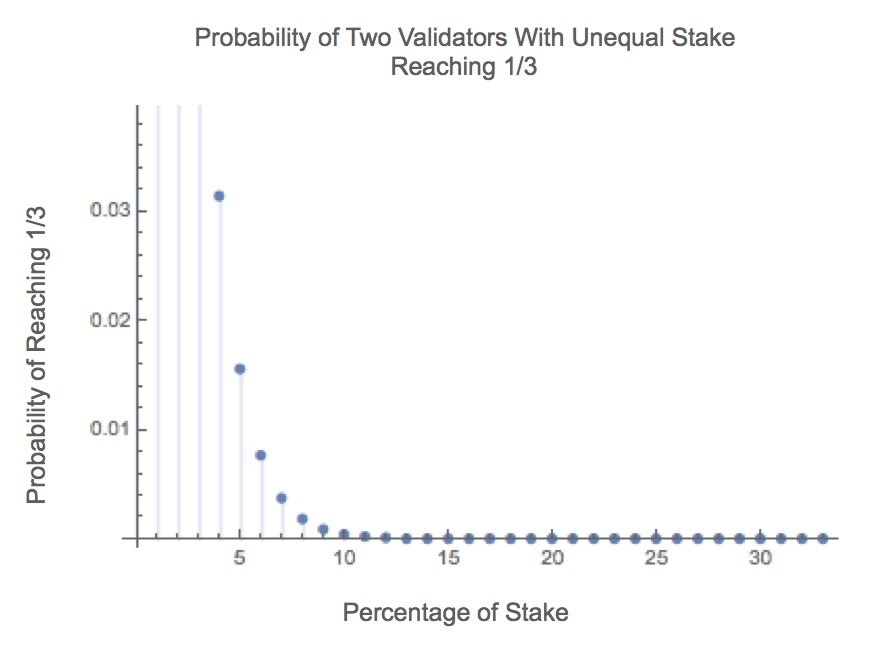
\includegraphics[scale=0.3]{images/2SkuVal.jpg}\newline\caption{Beta Binomial Distribution (probability density graph) conveying the probability of validator one reaching $\frac{1}{3}$ stake, when the two validators begin with skewed stake.}
\end{center} \\

In the following two scenarios, we model a system with 64 validators where the total amount of stake initially in the system is 2000 tokens and the reward to validators is one token. 

\begin{center}
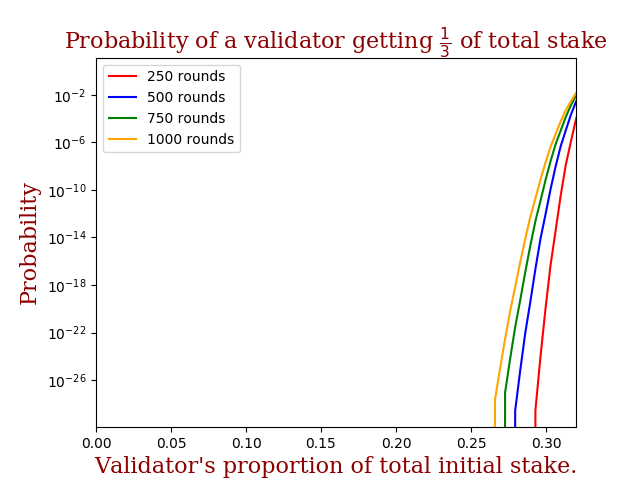
\includegraphics[scale=0.60]{images/Cons_reward_probability.png}\newline\caption{Probability that one validator starting at different initial proportions of stake reaches $\frac{1}{3}$ stake, in a system where each of the 64 validators begin with equal stake. In the 1000 rounds the probability of reaching $\frac{1}{3}$ is 2.19912034213425E-101 \%. \href{https://github.com/aparnakr/pos-analysis}{Modelled here.}}
\end{center}

\begin{center}
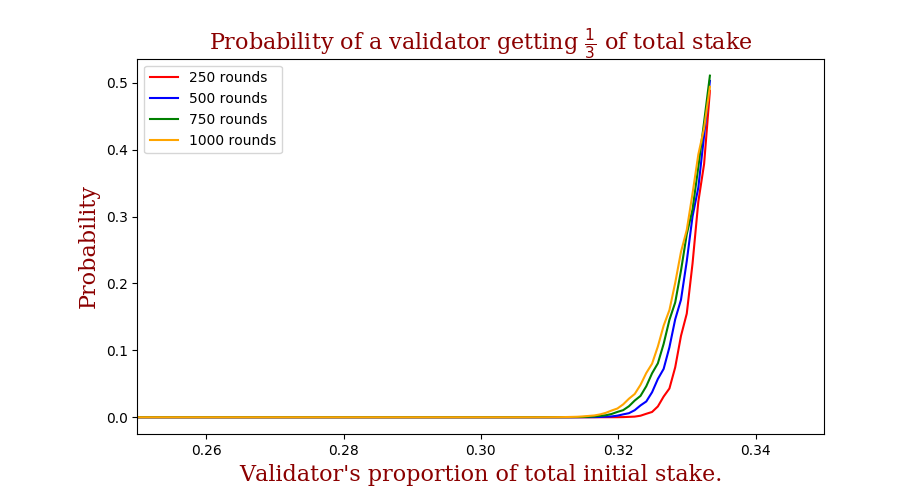
\includegraphics[scale=0.6]{images/Cons_reward_probability_non_log.png}\newline\caption{Probability that one validator starting at different initial proportions of stake reaches $\frac{1}{3}$ stake,in a system where each of the 64 validators begin with skewed stake.In the 1000 rounds the probability of reaching $\frac{1}{3}$ is 1.50938677083072E-130  \%. \href{https://github.com/aparnakr/pos-analysis}{Modelled here.}}
\end{center}
From the above graphs we see that the probability of any validator reaching the byzantine threshold is near zero when each validator has the same amount of stake. However, with a skewed distribution as seen in the second graph, validators with greater amounts of stake have a significantly higher likelihood of reaching $\frac{1}{3}$ stake.
\newline \newline 
Regardless of what the initial distribution is, section 4.1 proves that if the reward is a constant amount significantly less than the initial stake of each validator, the likelihood of any validator reaching the $\frac{1}{3}$ threshold is very low. 



\subsubsection{Calculating Expected Value}
Let the expected value of stake of a validator after $n$ rounds be $E[x_i^{(n)}]$.

$$E[x_0^{(i)}]= x_0^{(i)}$$

\begin{corollary} $$E[x_n^{(i)}] = x_0^{(i)}\frac{\Gamma_0 + n}{\Gamma_0}$$
\end{corollary}

\begin{proof}

Let $P(x_n^{(i)} = s)$ represent the probability of validator $i$ having stake $s$ in round $n$.
$$E[x_n^{(i)}] = \sum_{s \in values} \left(s + \frac{s}{\Gamma_0+n-1}\right)P(x_i = s)_{n-1} = E[x_{n-1}^{(i)}]\left(\frac{\Gamma_0+n}{\Gamma_0+n-1}\right)$$ 
$\Rightarrow E[x_{n-1}^{(i)}] = E[x_{n-2}^{(i)}] \left(\frac{\Gamma_0+n-1}{\Gamma_0+n-2}\right)$ and so on. Repeatedly substituting this in the above equation we can represent $E[x_{n}^{(0)}]$ as $E[x_n^{(i)}] = x_0^{(i)}\frac{\Gamma_0 + n}{\Gamma_0}$.
\end{proof}
\begin{theorem}
Consider a P\'olya Urn which starts with an initial stake distribution vector $X_0$. As the number of draws $n \rightarrow \infty$
\begin{equation}
    (\frac{x_n^{(1)}}{n},..,\frac{x_n^{(n)}}{n}) \rightarrow^D Dir(x_0^{(1)},..,x_0^{(n)}).
\end{equation}
\end{theorem} 
For the full proof, read \cite{Blackwell1973}.
\begin{center}
 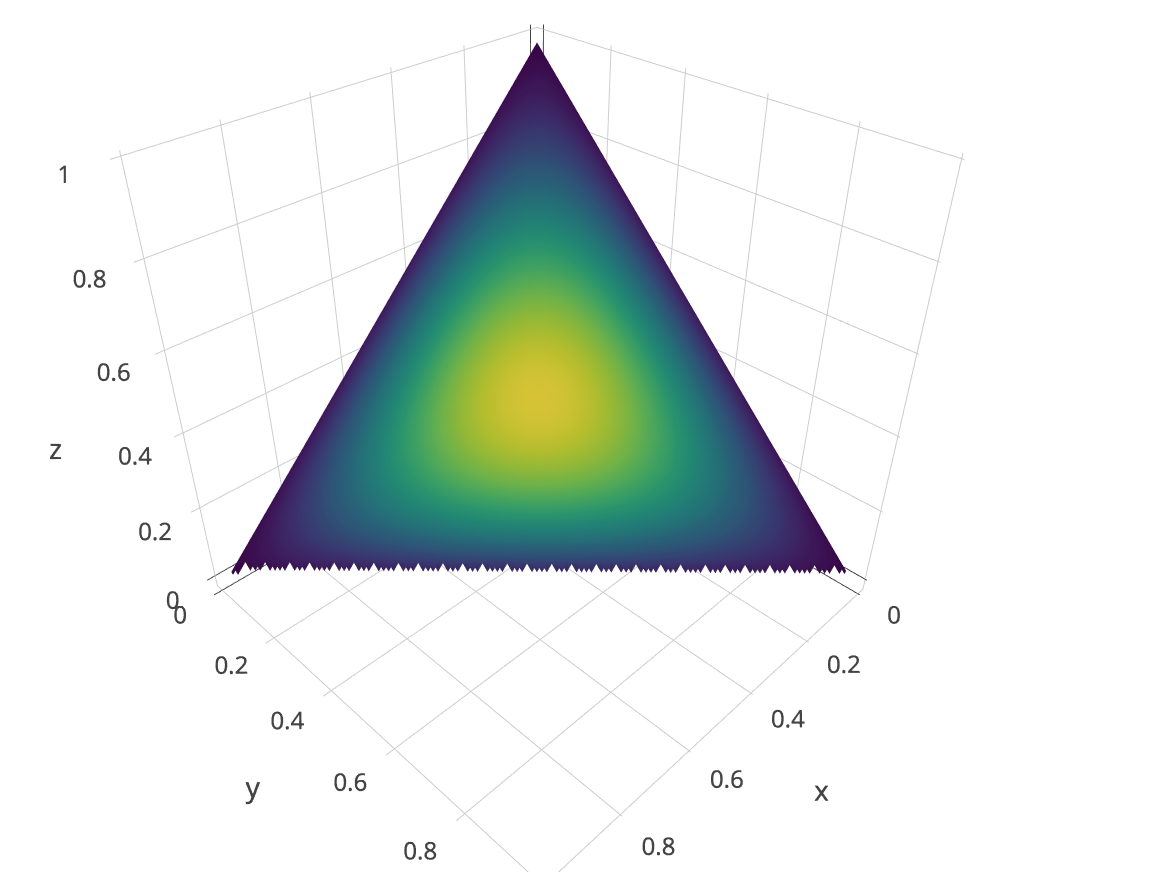
\includegraphics[scale=0.3]{images/dir_2_2_2.png}  
\end{center}
The above image shows a dirichlet graph of 3 validators all with initial equal stake.
\begin{center}
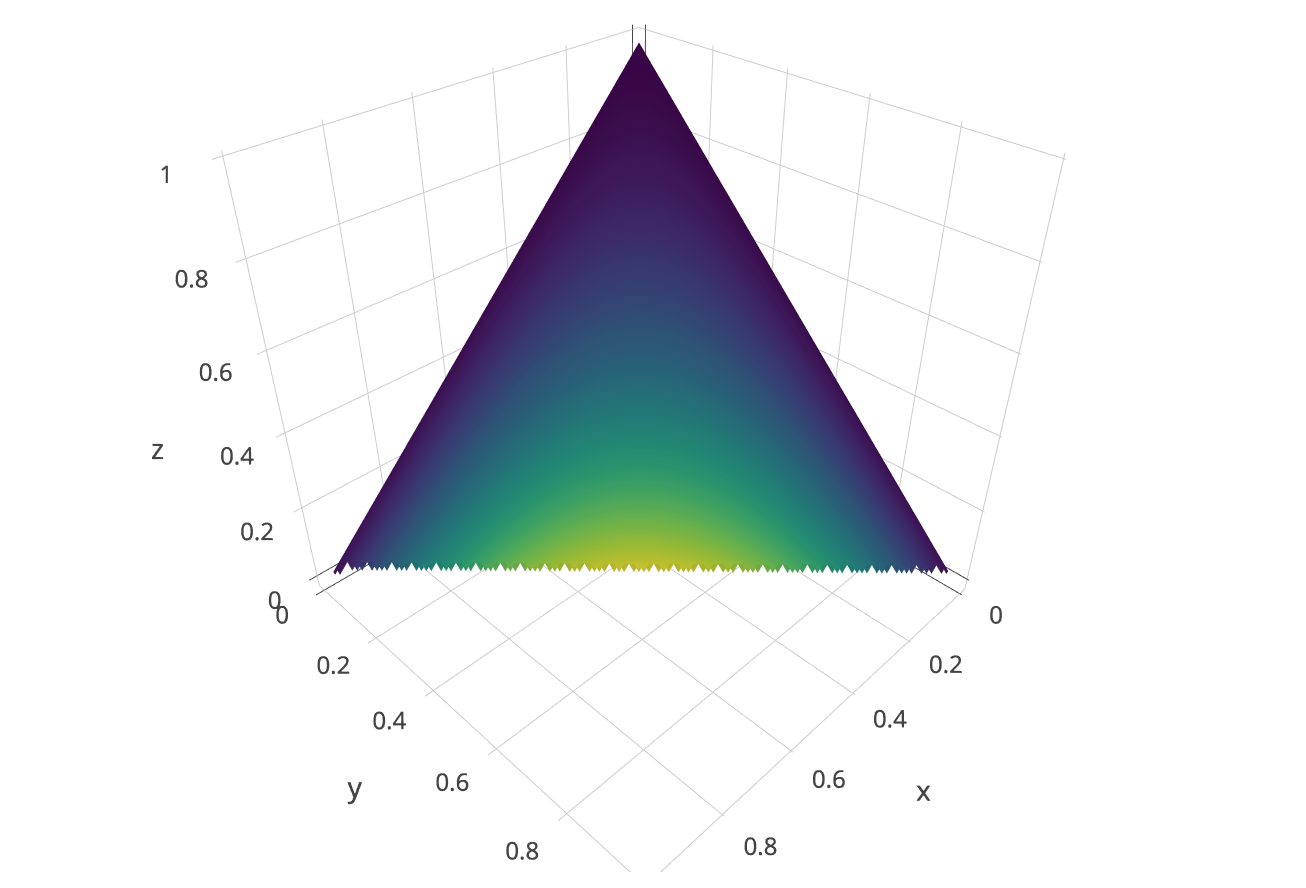
\includegraphics[scale=0.3]{images/dir_2_2_1.png}
\end{center}
The above image shows a dirichlet graph of 3 validators, 2 of which have equal stake and the other has slightly less stake than the others. 
\begin{center}
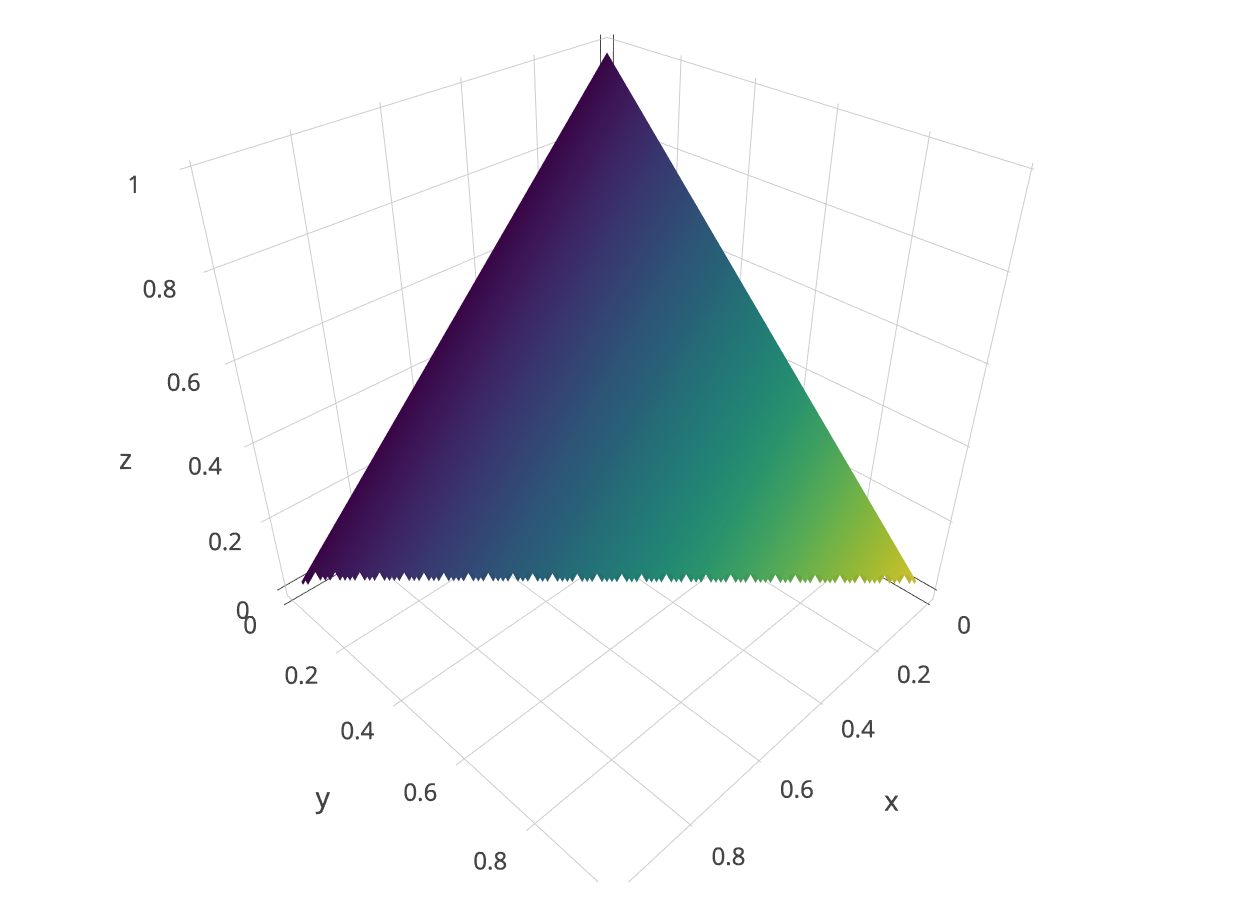
\includegraphics[scale=0.3]{images/dir_2_1_1.png}
\end{center}
The above image shows a dirichlet graph of 3 validators, 2 of which have equal stake and the other has slightly more stake than the others. 

\subsubsection*{Takeaway:}
 The P\'olya Urn model reveals that there is a near zero probabilistic likelihood of an actor getting to $\frac{1}{3}$ stake based off of stochastic randomness when the reward is some constant value. When stake is split evenly amongst validators, it is least likely that any single one reaches $\frac{1}{3}$. This indicates that a setup where each validator starts of with equal stake would be ideal. In future work, we will explore what happens when modifying the reward matrix, inflationary rewards, random rewards and if a breaking up of large stake is less secure from a probabilistic perspective. 

\section{Conclusion:}
In looking at the possibility of validators obtaining $\frac{1}{3}$ stake in the network, both intentionally and through stochastic randomness, we have exposed vulnerabilities in PoS regarding 33\% attacks. 
\newline
Key Findings: 
\begin{enumerate}
   \item It is possible to reach $\frac{1}{3}$ stake in the system when actively trying to do so as described by SRA
   \item There is a near zero probabilistic likelihood of an actor getting to $\frac{1}{3}$ stake based off of stochastic randomness dependent upon the number of validators 
\end{enumerate}\newline

\section{Further Research:}
Going forward, we will extend the P\'olya Urn model, looking into P\'olya's Urn with inflation. We plan to analyze the following 33\% attacks: Deposit Panic, Bribing Attacks, and P+ Epsilon Attacks. Other areas of research include looking into block rewards, punishments, tradeoffs between security and latency, delegated proof of stake, and a two token model. We aim to optimize constraints and parameters as a linear program to figure out how to optimize a PoS system.

\section{Appendix:}
\subsection{Intuition behind $\frac{1}{3}$ Byzantine Fault Tolerance}
To further expand on why $\frac{1}{3}$ byzantine faults provides a balance between consistency and availability, consider the case of $\frac{3}{4}$ fault tolerance. In this scenario, a distributed system could handle up to $\frac{1}{4}$ availability faults, meaning that if any more than $\frac{1}{4}$ of validators were offline, the system would not be able to function, but allows for $\frac{1}{2}$ consistency faults. Thus in the case of the $\frac{1}{3}$ threshold, the system can handle up to $\frac{1}{3}$ consistency faults, and also $\frac{1}{3}$ availability faults, allowing for this balance between consistency and availability that major PoS systems including Ethereum and Tendermint employ.


\newline
\newpage
\printbibliography

\clearpage

\end{document}

